\documentclass[9pt,spanish,aspectratio=1610]{beamer}
\usepackage[utf8]{inputenc}
\usepackage{amsmath}
\usepackage{graphicx}
\usepackage{amssymb}
\usepackage[spanish]{babel}
\spanishdecimal{.}
\usepackage{subfig}
\usepackage{fancyhdr}
\usepackage{pstricks}
\usepackage[ruled]{algorithm2e}
%\usepackage{ragged2e}
%\usepackage[natbibapa]{apacite}
% \bibliographystyle{apacite} % This is the style you should use with `apacite`.
%\justifying
\DeclareMathOperator{\atantwo}{atan2}
\newcommand\ddfrac[2]{\frac{\displaystyle #1}{\displaystyle #2}}
\usetheme{Boadilla}
\setbeamercovered{transparent}
\beamertemplatenavigationsymbolsempty
\setbeamertemplate{frametitle}
{
  \leavevmode
  \hbox{
  \begin{beamercolorbox}[wd=0.6\paperwidth,left]{frametitle}
    \usebeamerfont{frametitle}\insertframetitle
  \end{beamercolorbox}
  \begin{beamercolorbox}[wd=0.4\paperwidth,center]{frametitle}
    \usebeamerfont{frametitle}\hfill\small{\thesection. \insertsection}
  \end{beamercolorbox}
  }
}
\setbeamertemplate{footline}
{
  \leavevmode%
  \hbox{%
    \begin{beamercolorbox}[colsep=-0.5pt,wd=.33\paperwidth,ht=3ex,dp=1.5ex,center]{author in head/foot}%
      \usebeamerfont{author in head/foot}\insertshortauthor~~ (\insertshortinstitute)
    \end{beamercolorbox}%
    \begin{beamercolorbox}[colsep=-0.5pt,wd=.34\paperwidth,ht=3ex,dp=1.5ex,center]{date in head/foot}%
      \usebeamerfont{author in head/foot}\insertshorttitle
    \end{beamercolorbox}%
    \begin{beamercolorbox}[colsep=-0.5pt,wd=.33\paperwidth,ht=3ex,dp=1.5ex,right]{author in head/foot}%
      \usebeamerfont{author in head/foot}\insertshortdate{}\hspace*{2em}\scriptsize{\insertframenumber{}}\hspace*{1ex}
    \end{beamercolorbox}
  }
}

\begin{document}
\renewcommand{\tablename}{Tabla}
\renewcommand{\figurename}{Figura}

\title[Object Recognition using Fault Reconstruction Techniques]{Object Recognition by Physical Properties Detection using Fault Reconstruction Techniques}
\author[Marco Negrete and Jesús Savage]{Marco Negrete and Jesús Savage}
\date[RFC-MathWorks Support for Research Projects 2020]{Proposal for the RCF and MathWorks Support for Research Projects 2020}
\institute[FI, UNAM]{Faculty of Engineering, UNAM}

\begin{frame}
\titlepage
\end{frame}

\begin{frame}\frametitle{Objectives and Goals}
  \textbf{Objectives:}
  \begin{itemize}
  \item Applying model based fault signal reconstruction algorithms (MBFRA) to improve manipulation tasks in domestic service robots.
  \item Use an sliding mode observer to estimate the weight of the object being manipulated by the robot.
  \item Implement the developments in ROS nodes.
  \end{itemize}

  \textbf{Goals:}
  \begin{itemize}
  \item Obtain a model of the manipulator using Simscape (\textbf{check})
  \item Implement a system identication algorithm  (\textbf{uncheck})
  \item Design a sliding mode observer to estimate the joint velocities (\textbf{check})
  \item Use the output injection term to estimate the weight being carried by the robot (\textbf{check})
  \item Export estimators from Matlab to ROS nodes (\textbf{uncheck})
  \end{itemize}
\end{frame}

\begin{frame}\frametitle{Simscape model}
  \begin{itemize}
  \item Model was obtained from the original version of Justina's urdf (see left figure).
  \item As a first step to address the problem, we considered only a 2DOF manipulator, i.e., all joints were set to ``fixed'' except the shoulder and elbow pitch. Right figure shows this simplified model. 
  \end{itemize}
  \begin{columns}
    \begin{column}{0.5\textwidth}
      \begin{figure}
        \centering
        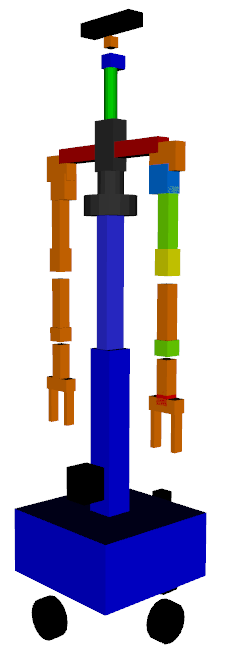
\includegraphics[width=0.3\textwidth]{Figures/justina_urdf.png}
      \end{figure}
    \end{column}
    \begin{column}{0.5\textwidth}
      \begin{figure}
        \centering
        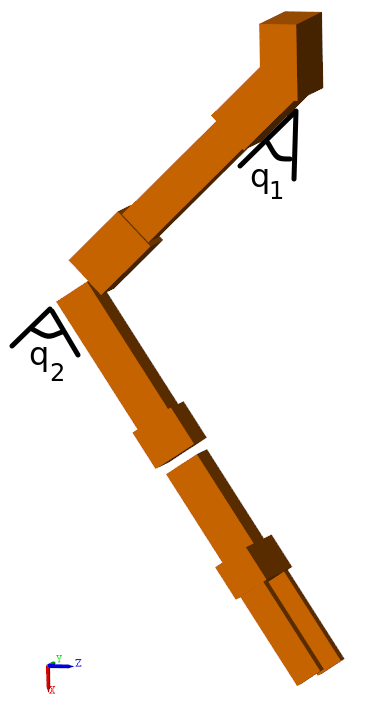
\includegraphics[width=0.4\textwidth]{Figures/simplified_model.png}
      \end{figure}
    \end{column}
  \end{columns}
\end{frame}

\begin{frame}\frametitle{Dynamic model}
  Sliding Mode Observers (SMO) were proposed as the method to estimate the mass of the manipulated object. Thus, we need first to obtain the dynamic model.\\
  From the Langrangian of the manipulator, a dynamic model of the following form can be obtained:
  \begin{equation}
    M(q)\ddot{q} + C(q, \dot{q})\dot{q} + B\dot{q} + G(q) = u
    \label{eq:lagrangian}
  \end{equation}
  where $q\in \mathbb{R}^2$ are the joint angles, $M(q)\in \mathbb{R}^{2\times 2}$ is the inertia matrix, $C(q,\dot{q})\in \mathbb{R}^{2\times 2}$ is the Matrix of Coriollis forces, $B\dot{q}\in \mathbb{R}^2$ is the vector of friction forces, $G(q)\in\mathbb{R}^2$ is the vector of gravitational forces and $u$ is the input torque, considered as control signal. \\
  To design a SMO is necessary to write the model in variable states form. Let $x_1 = [q_1\;q_2]^T$ and $x_2 = [\dot{q}_1\;\dot{q}_2]^T$ be the state variables. Then (\ref{eq:lagrangian}) can be written as:
  \begin{eqnarray}
    \dot{x}_1 &=& x_2\label{eq:model1}\\
    \dot{x}_2 &=& -M^{-1}(q)\left(C(q, \dot{q})\dot{q} + B\dot{q} + G(q) - u\right)\label{eq:model2}
  \end{eqnarray}
  If uncertainties and disturbances are considered, then (\ref{eq:model2}) can be written as
  \begin{equation}
    \dot{x}_2 = f(x_1, x_2, u) + g(x_1, x_2, u)
  \end{equation}
  where $f(x_1, x_2, u) = -M^{-1}(q)\left(C(q, \dot{q})\dot{q} + B\dot{q} + G(q) - u\right)$ is the nominal part and $g(x_1, x_2, u)$ contains all terms related to uncertainties and disturbances. If the system is correctly identified, then $g(x_1, x_2, u)$ corresponds only to disturbances. 
\end{frame}

\begin{frame}\frametitle{Sliding Mode Observer}
  If a SMO is used to estimate the joint speeds, the unknown term $g(x_1, x_2, u)$ can be reconstructed by an appropriate filtering of the output error injection term. The following observer was used:
  \begin{eqnarray}
    \dot{\hat{x}}_1 &=& \hat{x}_2 + z_1\label{eq:model1}\\
    \dot{\hat{x}}_2 &=& f(x_1, \hat{x}_2, u) + z_2\label{eq:model2}
  \end{eqnarray}
  where $z_1$ and $z_2$ are the output error injection terms calculated as
  \[ z_1 = \left[\begin{tabular}{c}
      $\lambda\vert q_1 - \hat{q}_1\vert ^{1/2}sign(q_1 - \hat{q}_1)$ \\
      $\lambda\vert q_2 - \hat{q}_2\vert ^{1/2}sign(q_2 - \hat{q}_2)$
    \end{tabular}\right]
  \]
\end{frame}
\end{document} 
